\section{Integration of Distributed Energy Resources in Distribution System}
With the growing population, and increasing modernization and industrialization, the global demand is estimated to increase drastically, more than triple by the ends of this century \cite{INTRO1}. The present power industry is faced with the great challenge of balancing power generation with this increasing demand. In 2017 an estimated 4 trillion kilowatt hours of electricity was generated to meet the demands of the United States \cite{EIA2018}. Table \ref{tab:IN1} shows the percentage of the different sources of generation in the U.S. for the year 2017. The data used in the Table is collected from \cite{EIA2018}.

\begin{table}[ht]
\label{tab:IN1}
\caption[U.S. electricity generation by source, amount, and share of total in 2017]{U.S. electricity generation by source, amount, and share of total in 2017 \cite{EIA2018}}
\centering
\begin{tabular}{|c|c|c|}
\hline
Energy source & Billion kWh & Share of total \\ \hline
Total - all sources & 4,034 &  \\ \hline
Fossil fuels (total) & 2,536 & 62.90\% \\ \hline
Natural gas & 1,296 & 32.10\% \\ \hline
Coal & 1,206 & 29.90\% \\ \hline
Petroleum (total) & 21 & 0.5\% \\ \hline
Petroleum liquids & 12 & 0.3\% \\ \hline
Petroleum coke & 9 & 0.2\% \\ \hline
Other gases & 12 & 0.3\% \\ \hline
Nuclear & 805 & 20.0\% \\ \hline
Renewables (total) & 687 & 17.0\% \\ \hline
Hydropower & 300 & 7.4\% \\ \hline
Wind & 254 & 6.3\% \\ \hline
Biomass (total) & 63 & 1.6\% \\ \hline
Wood & 41 & 1.0\% \\ \hline
Landfill gas & 12 & 0.3\% \\ \hline
Municipal solid waste (biogenic) & 7 & 0.2\% \\ \hline
Other biomass waste & 3 & 0.1\% \\ \hline
Solar (total) & 53 & 1.3\% \\ \hline
Photovoltaic & 50 & 1.2\% \\ \hline
Solar thermal & 3 & 0.1\% \\ \hline
Geothermal & 16 & 0.4\% \\ \hline
Pumped storage hydropower & -6 & -0.2\% \\ \hline
Other sources & 13 & 0.3\% \\ \hline
\end{tabular}
\end{table}

From the table \ref{tab:IN1} it is evident that the current energy sources mostly rely on natural gas and coal. These are resources that do not renew at a sufficient rate to allow sustainable extraction. The increased power demand combined with the non-renewable nature of the energy resources and their adverse effect on the environment necessitates the incorporation of new and alternative resources to meet the future demand. This has been a significant drive for renewable distributed energy resource (DER) integration into the grid \cite{khan2009review,bignucolo2008radial,series2009microgrids}. With the growth in power demand the penetration of distributed energy resource in the distribution system is rising. This trend of adding energy resources in the distribution system is changing the current infrastructure of modern power systems. Fig. \ref{fig:NEW_GRID} shows this transformation of the power grid and what it might look like in the near future. 

\begin{figure}[!h]
\centering
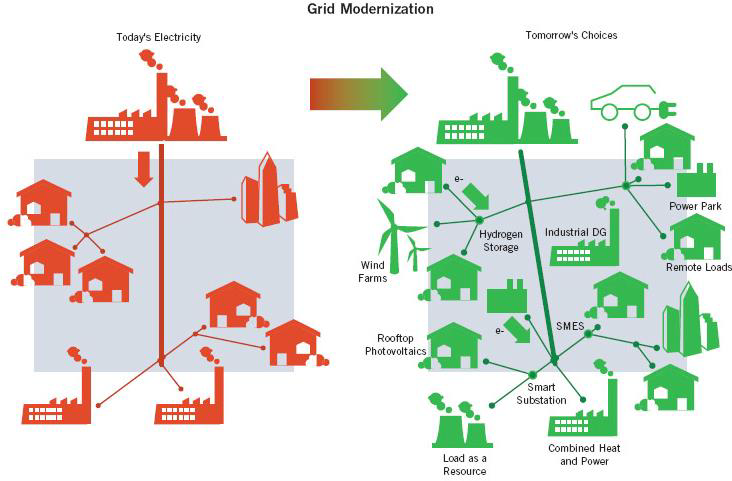
\includegraphics[width=0.85\linewidth]{figs/NEW_GRID.png}
\caption[Power grid modernization.]{Power grid modernization.\cite{NEW_GRID}}
\label{fig:NEW_GRID}
\end{figure}

With the integration of DERs power is no longer only generated in bulk at generation facility and then through transmission and distribution supplied to the consumer. DERs make it possible to generate power near the demand. This increases system stability and reduces system loss as power does not need to travel far to reach the source. DERs can be divided into distributed generation (DG) and distributed energy storage (DES). 

\subsection{Distributed Generation}
Distributed generation is an approach that employs appropriate small and medium scale electricity generation resources near the consumer. Non-renewable fuel based distributed generation technologies and dispatchable renewable distributed generation has been a part of the grid for many years. In recent years the incorporation of variable renewable energy based DG has increased significantly. There are mainly two types of variable renewable DGs used in the distribution grid.
\begin{enumerate}
    \item Solar Energy Based DGs
    \item Wind Energy Based DGs
\end{enumerate}
Besides these, biomass, small scale hydro and combined heat and power are some of the prominent distributed generation plants being added to the grid. Fig. \ref{fig:GROWTH_EIA} shows the current trend as well as the projected future of electricity generation by source. It is evident from the figure that renewable generation sources will keep on increasing in the grid. 

\begin{figure}[!h]
\centering
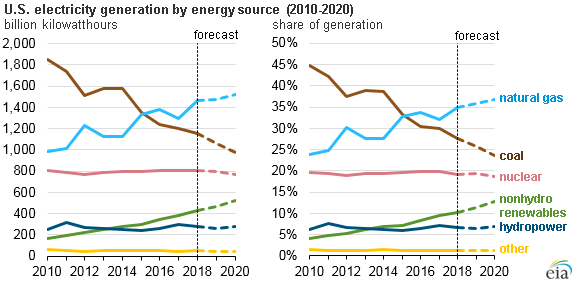
\includegraphics[width=0.85\linewidth]{figs/GROWTH_EIA.png}
\caption[Us electricity generation by energy source.]{Us electricity generation by energy source.\cite{EIA2018}}
\label{fig:GROWTH_EIA}
\end{figure}

\subsection{Distributed Energy Storage}
Energy storage can provide backup power and increase grid stability by mitigating the effects of variable renewable generation in the grid. It can also be used to store energy during relatively low demand and release it back during high demand periods. There are various energy storing methods currently used in the grid, including \cite{GE1}:
\begin{itemize}
    \item \textbf{Pumped Hydro:} In times of low demand and high generation electricity is used to pump water in a storage reservoir. During high demand, the stored water is used to generate power.
    \item \textbf{Compressed Air:} During low demand electricity is used to store compressed air up to 1,000 Psi. Then it is used to generate during low demand.
    \item \textbf{Batteries:} Batteries store electricity in the form of chemical energy. Similar to the previous approaches electricity is stored during low demand and released during high demand.
    \item \textbf{Flywheels:} Flywheel uses electricity to store rotational kinetic energy. During low demand, a motor is used to rotate the flywheel and store kinetic energy. During high demand, this kinetic energy is used to rotate a generator and produce power.
    \item \textbf{Thermal Storage:} During times of low demand electricity is used to store thermal energy. Then during high demand, the stored energy is used for heating and cooling applications.
\end{itemize}

As of June 2016, the U.S. had over 21.6 GW of rated power in energy storage. Most of the projects are Electro-chemical energy storage projects. Pumped hydro storage represents the majority capacity of the currently available storage. Fig. \ref{fig:ES_INCREASE} shows the growth of energy storage installation in the grid. Between the years 2008 – 2016 the U.S. has installed 1.17 GW new energy storage capacity in the grid. 

\begin{figure}[!h]
\centering
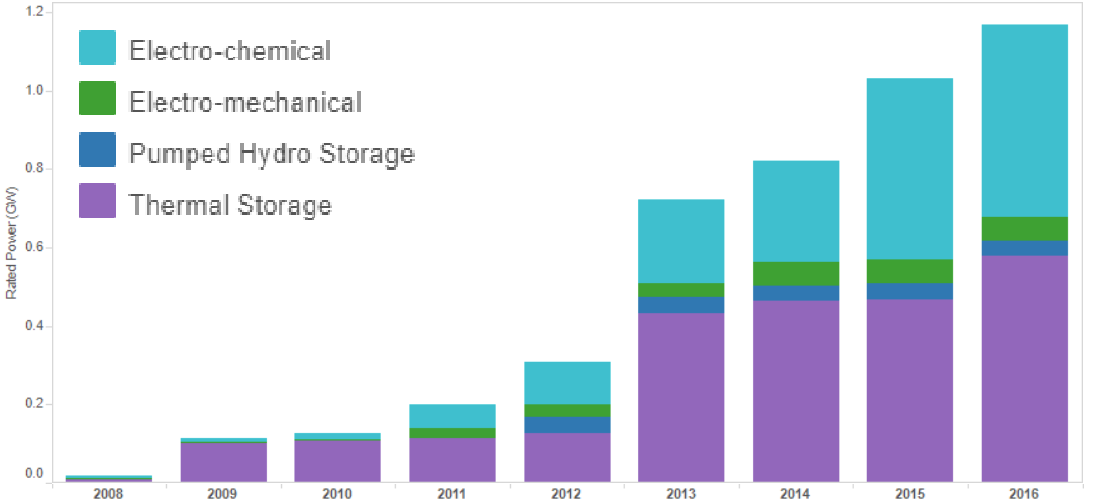
\includegraphics[width=0.85\linewidth]{figs/ES_INCREASE.png}
\caption[Recently installed grid energy storage in the U.S.]{Recently installed grid energy storage in the U.S \cite{GE2}}
\label{fig:ES_INCREASE}
\end{figure}


\section{Issues Due to High Penetration of DERs in Distribution system}
The current power grid was designed to accommodate unidirectional power flow. This was an efficient design to distribute power from central transmission to distribution feeders to the loads \cite{HPPV}.  With the introduction of DGs, the traditional design has to face some new challenges. The existing distribution system components were not designed to accommodate bidirectional power flow \cite{HPPV}. Therefore, concerns are arising regarding the increased penetration of DGs. This is a vital research field. This field is getting more attention as more DGs are incorporated into the grid. 

The potential impact of integration of DGs in the distribution system is affected by many different parameters. The location and rating of the DG, the regulation and protection equipment present in the system, the stiffness of the feeder, etc. play a significant role in the impact of the DG. Moreover, the variability of the non-dispatchable variable DGs also plays a significant role in the negative impact the DGs might have on the feeder. This chapter will present a review of the potential impacts of DG integration, mostly focusing on voltage regulation issues.

\subsection{General Potential Impacts}
There are a lot of potential impacts that may happen in a distribution grid with a high penetration of DGs. This brief review presents a small part of the impacts. In this section, some of the general system level impacts are stated with references that deeply explain the phenomenon. Some of the impacts may be:
\begin{itemize}
    \item Voltage ride through. \cite{GPI1}
    \item Tripping of multiple DGs.\cite{GP2}
    \item Reverse power flow causing equipment malfunction. \cite{GP3}
    \item Resonance caused by multiple inverter output capacitance. \cite{GP4}
    \item DC injection. \cite{GP5}
    \item Protection system coordination. \cite{GP3}
    \item Line overloading. \cite{GP6}
    \item High penetration of DG can have impact on transformer insulation. \cite{GP4}
\end{itemize}
The effects of DG integration can appear at any level of penetration but as the DG generation start to overcome the demand of the nearby loads the effects start to become more prominent \cite{Th_ali}.

\subsection{Technical potential impact}
Besides these, there are some technical potential impacts that need to be considered.

\subsubsection{Impacts on Power Quality}
“Power quality is a set of electrical boundaries that allow a piece of equipment to function in its intended manner without significant loss of performance or life expectancy” \cite{TPI1}. Another definition according to IEEE standard 1159 – 2009 defines power quality as “a wide variety of electromagnetic (EM) phenomena that characterize the voltage and current at a given time and a given location on the power system” \cite{TPI2}.  Power quality has become a vital topic in recent years as the use of power electronic devices in the grid has increased. These have introduced the following types of power issues in the system.

According to IEEE standard 1159 – 2009, electromagnetic compatibility (EMC) is defined as “the ability of a device, equipment or system to function satisfactorily in its electromagnetic environment without introducing intolerable electromagnetic disturbances to anything in that environment.”  EMC has been accepted by the international community of the International Electro-technical Commission (IEC) to describe power quality phenomena \cite{TPI2}. Both the standard IEEE 1159 – 2009 and the IEC 61000-4-7 standard give a detailed description of different electromagnetic (EM) phenomena pertaining to power quality. The IEEE 1159 – 2009 categorize these phenomena into seven main categories and that further branch into subcategories as stated below:
\begin{enumerate}
    \item Transients
    \item Short-duration root-mean-square (rms) variations
    \item Long duration rms variations
    \item Imbalance in steady state
    \item Waveform distortion
    \item Voltage fluctuations 
    \item Power frequency variations
\end{enumerate}

\subsubsection{Islanding}
Islanding or more specifically unintentional islanding is a possible threat of DG integration. Islanding occurs when a section of the feeder is isolated, and the DG present in that section continues to feed the local load. This can lead to some adverse effects. If the protection system in the distribution network is designed to reestablish the circuit after clearance of temporary fault, the active DG might be reconnected to the grid out of phase. This can cause damage to the DG and equipment on the feeder \cite{ILAND_1}. There is also the risk of workers working on an unintentionally islanded system without knowing the system in energized \cite{ILAND_1}. Additionally, the utility cannot control the power quality of the DGs in the islanded system. The protection system in place in the islanded system may not be adequately coordinated to work without the presence of the grid. This can lead to permanent faults in the islanded sections with lower current values than usual because the protection coordination did not respond \cite{ILAND_2}.

\subsubsection{Voltage regulation}
The impact of DG on voltage variation is mostly prevalent in distribution networks. The distribution networks are radial. Let us consider the radial feeder shown in 
Fig. \ref{fig:VR1} In \cite{VR1} a study was done inserting PV system in different nodes along the feeder. Fig. \ref{fig:VR2} Shows how the voltage level is affected by integrating a PV plant at different positions of the feeder. It can be seen that PV addition near the end of the line causes a greater disturbance on the line voltage compared to PV inserted close to the substation. So depending on the capacity and the point of integration, a DG can take the voltage limit outside standards such as those in ANSI C84.1 and IEEE 1547 \cite{VR2}. 

\begin{figure}[!h]
\centering
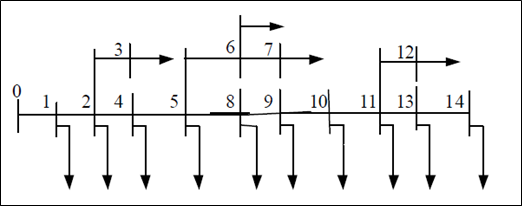
\includegraphics[width=0.85\linewidth]{figs/VR1.png}
\caption[One line diagram of a radial feeder]{One line diagram of a radial feeder.\cite{VR1}}
\label{fig:VR1}
\end{figure}

\begin{figure}[!h]
\centering
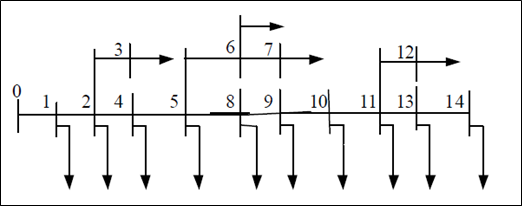
\includegraphics[width=0.85\linewidth]{figs/VR1.png}
\caption[Node voltage of PV accessing at different positions]{Node voltage of PV accessing at different positions.\cite{VR1}}
\label{fig:VR2}
\end{figure}

In addition to the change in the line voltage distribution, the presence of a variable DG in the system can cause a disturbance in the system voltage. Fig. \ref{fig:VR3} shows the load of a substation with and without a variable DG \cite{GKA11}. The variable DG, in this case, is a PV plant. In the figure, the normal demand on the substation is in black, and the demand with the presence of variable DG is in red. It can be seen that the red profile has a very irregular pattern. This voltage fluctuation can cause increased operation of the voltage regulation devices (OLTC, SCB and SVR). As these are mechanical devices increased operations can decrease their life expectancy.
 
\begin{figure}[!h]
\centering
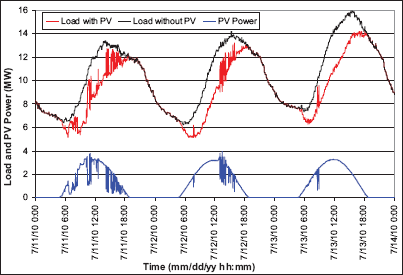
\includegraphics[width=0.7\linewidth]{figs/VR3.png}
\caption[Substation load with and without DG.]{Substation load with and without DG \cite{GKA11}.}
\label{fig:VR3}
\end{figure}
 

Fig. \ref{fig:VR4} shows the normal switching profile of a substation step voltage regulator without PV and Fig. \ref{fig:VR5} shows the switching profile with PV. As it can be seen from the figures, the presence of the variable DG caused much more switching operations. Moreover, DG near loads may increase the voltage in that zone beyond the limits set by standards. This increase in voltage may not trigger the voltage regulation devices as the nodes the devices are monitoring can stay within limits. Therefore, the controls of the devices may need to be upgraded as DG penetration in the grid increases \cite{IEE13}. These impacts can increase costs due to tear and ware in switching devices, decreases equipment life due to over-voltage and need for more power factor correction equipment. 

\begin{figure}[!h]
\centering
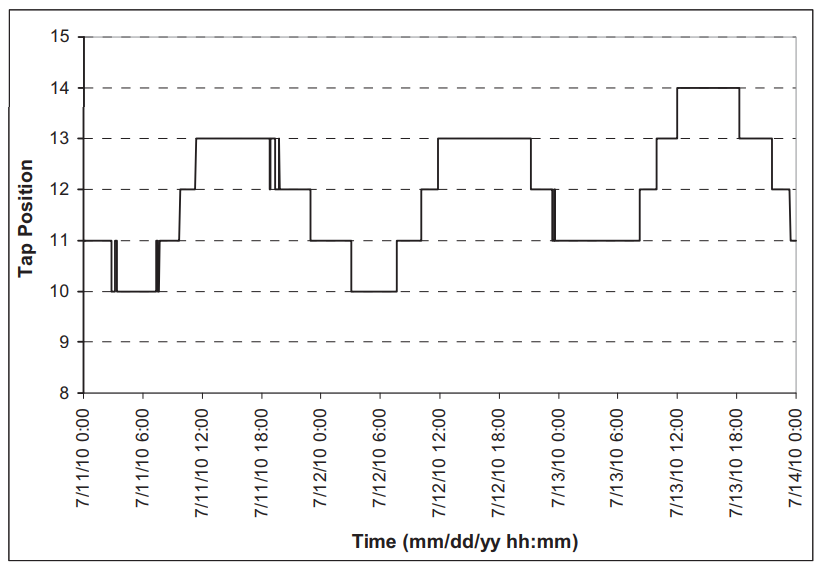
\includegraphics[width=0.85\linewidth]{figs/VR4.png}
\caption[Substation transformer tap changer position without DG]{Substation transformer tap changer position without DG \cite{GKA11}.}
\label{fig:VR4}
\end{figure}
 
 \begin{figure}[!h]
\centering
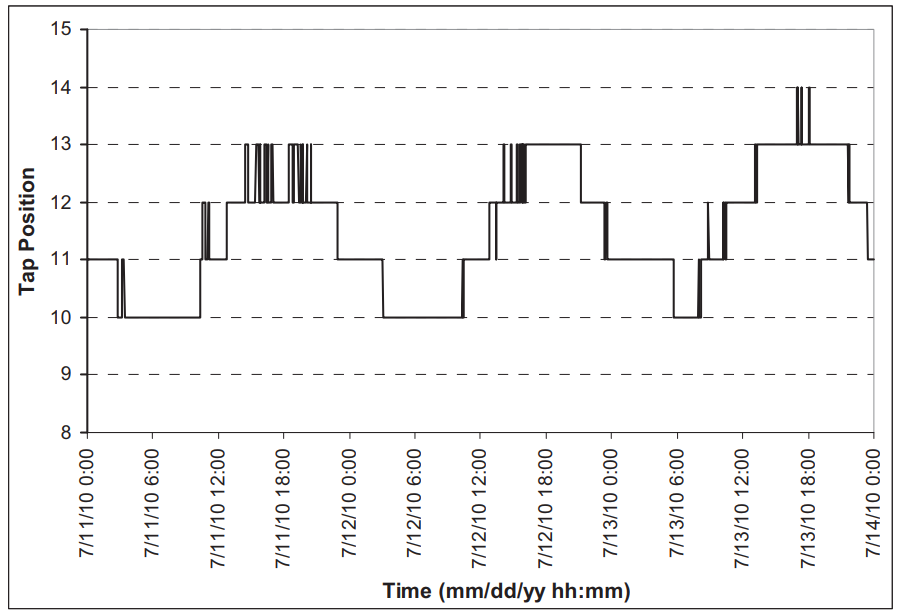
\includegraphics[width=0.85\linewidth]{figs/VR5.png}
\caption[Substation transformer tap changer position with DG.]{Substation transformer tap changer position with DG \cite{GKA11}.}
\label{fig:VR5}
\end{figure}

\subsubsection{System protection impacts}
The protection system of the distribution grid has been designed for unidirectional power flow. The integration of DG will require upgrading the protection system for better protection coordination. Usually, distribution systems employ protection schemes that consist of fuses, circuit breakers, sectionalizes, and automatic restoration devices that are coordinated in the load direction to operate with a minimum number of customers affected \cite{PRO1}. This coordination does not account for the integration of DG in the system. The integration of DG introduces more sources in the feeder to contribute to the fault current. Depending on the fault location, rating of DG and protection system installed, many problems could arise. Some of the possible problems are listed below.
\begin{enumerate}
    \item Fault level modification
    \item Blinding of Protection
    \item Sympathetic tripping
    \item Reduction in reach of distance relay
    \item Sensitivity reduction of high impedance fault detection
\end{enumerate}
Detailed analysis of the problems can be found in \cite{PRO2}.




\section{ADMS (Advanced Distribution Management System)}
From the previous discussion, it is evident that increased DER penetration is bringing some complex problems to be solved. To combat these emerging issues, new technology is being added to the aging infrastructure of the traditional power grid. These new technologies are known as "smart grid" technologies. The future evolving grid or “smart grid” has to incorporate information technology, communication technology and advanced control with power engineering. Another major aspect of the smart grid is control automation. The smart grid has to be self -healing and capable of maintaining system stability in case of system change and anomalies. Moreover, the grid of the future has to enable its stakeholders to realize new ways of performing energy transactions across the system while making sure it is financially viable and beneficial for both parties \cite{SG1}. To maximize the utilization of these new resources and data available a proper management system is required. The concept of ADMS (advanced distribution management system) is introduced to handle this task. The concept of ADMS is still an evolving topic, and different sources define the components present in an ADMS system differently. However irrespective of the internal architecture there are three major functions a modern ADMS system should be able to perform \cite{ADMS_1}.
\begin{itemize}
    \item Monitor and operate: An ADMS system should be capable of wide area monitoring and operations. Utilities use SCADA systems to monitor the state of the grid from a central location. SCADA provides the current status of different protection systems, alarms and metering devices to aid the operator in system operation.
    \item Analyze and Optimize: Analysis and optimization are done using the distribution network applications included with the ADMS. The included applications vary between different ADMS providers. The main purpose here is to optimize the use of available resources without jeopardizing system stability.
    \item Track and Restore: With the integration of DERs and introduction of reverse power flow the fault characteristics of a distribution grid has changed drastically. Proper identification of fault location very complex problem. ADMS solutions provide different components like outage management system, auto system restoration system, fault identification system, etc. to aid the utilities in fault detection and system restoration.
\end{itemize}
As the ADMS is an evolving technology, the ADMS architecture is defined differently by various sources. Fig. \ref{fig:ADMS_ARCH} shows the ADMS architecture proposed by the United States department of energy. The shaded region represents the sections which are still being actively developed and researched. Integrating these aspects with the existing management system is the major challenge of designing a modern ADMS system. Short descriptions of the different components of the ADMS architecture proposed by the United States department of energy are given below \cite{ADMS_2}:

\begin{figure}[!h]
\centering
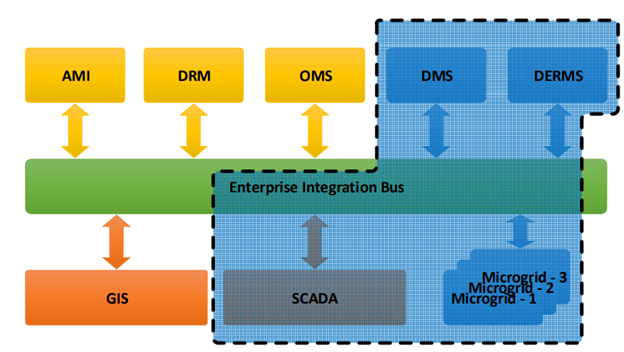
\includegraphics[width=0.85\linewidth]{figs/ADMS_ARCH.png}
\caption[ADMS architecture]{ADMS architecture. \cite{ADMS_2}}
\label{fig:ADMS_ARCH}
\end{figure}

 \begin{itemize}
     \item \textbf{AMI:} AMI represents the advanced metering infrastructure. The AMI is responsible for aggregating different measured data and sending it to the utility.
     \item \textbf{DRM:} DRM stands for dispatchable resource management. It chooses the most cost-effective way to modulate the traditional dispatchable resources to meet the current demand.
     \item \textbf{OMS:} The Outage Management System is in charge of managing the process of restoration after an outage has occurred in the grid. It is in charge of detecting incidents and automatically reconfiguring the network to have the least outage possible. It also deals with customer calls and crew management to restore service.
     \item \textbf{GIS:} A geographical information system(GIS) lets the utility analyze, interpret and visualize data based on geographical location. This helps the operators in real-time monitoring of the system. It also helps the operators to understand patterns and trends in the system.
     \item \textbf{SCADA:} The purpose of SCADA (supervisory control and data acquisition) is to monitor and control the system based on the data collected from different sources. SCADA is used for high-level supervision and management.
     \item \textbf{DMS:} DMS stands for Distribution Management System. This is used for managing different resources at the distribution level.
     \item \textbf{DERMS:} DERMS stands for Distributed Energy Resource Management System. DERMS work in conjunction with the DMS to ensure the efficient use of DERs in the distribution system. It can be viewed as a subsystem of the DMS in charge of DERs.
     \item \textbf{Microgrid:} Microgrids are entities capable of operating self-sufficiently with or without grid connection. The utility or another third party can own microgrids. The microgrids can be operated as a self-sufficient zone in times of high demand and faults.
 \end{itemize}

\subsection{DERMS (Distributed Energy Resource Management System)}
As this report focuses on components of DERMS, this concept is explained in more detail. The conventional power grid had an unpredictable and varying load profile. To counter this, the traditional grid used the dispatchability of traditional power plants and spinning reserves to maintain reliable power flow. It is also clear from the discussions thus far that the integration of distributed generation resources in the distribution system is increasing rapidly. As variable DG integration increases in the grid, the unpredictability of the grid rises drastically. The traditional approach of keeping spinning reserves are not only expensive but also inefficient to deal with this modern varying grid. Storage technology can play a crucial role in decreasing the variability of the grid \cite{USD13}. With recent advances in energy storage, utilities are considering deploying energy storage rated from 2kWh to 50 MWh in the distribution level \cite{Cle12}. Medium to small scale energy storage deployed near the consumer end lets the utilities provide better voltage control, renewable integration and reduced distribution losses while providing them the means to absorb fluctuation in prices and load. Moreover, with real-time pricing, the consumer can optimize the use of their energy storage and minimize electricity cost by taking advantage of the fluctuating price \cite{BPR11,PMv13,ASB17}.
Optimizing the use of energy resources can lead to a lower cost. However, grid voltage stability and constraints cannot be compromised to gain the optimal solution. Integration of DGs produce challenges for maintaining system voltage stability. Another major concern is the new complexities that arise in properly protecting the system. The traditional protection schemes are not adequate in maintaining optimal system protection. To manage these new DERs at the distribution level, the concept of DERMS (Distributed Energy Resource Management System) has been introduced. Fig. \ref{fig:DERMS_ARCH} shows functions of a DERMS system. 

\begin{figure}[!h]
\centering
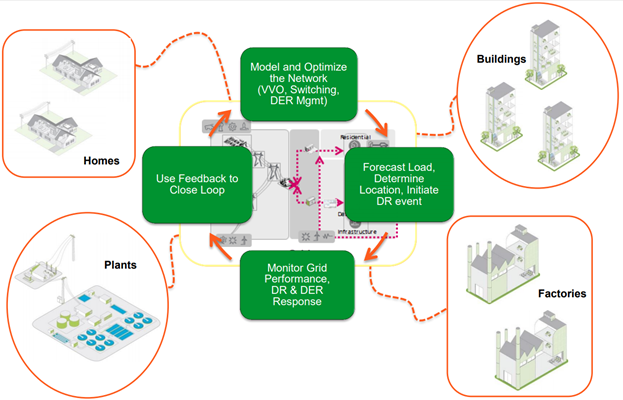
\includegraphics[width=0.85\linewidth]{figs/DERMS_ARCH.png}
\caption[Functions of DERMS.]{Functions of DERMS. \cite{DERMS_1}}
\label{fig:DERMS_ARCH}
\end{figure}

As seen in Fig. \ref{fig:DERMS_ARCH} the DERMS system achieves it's purpose by following certain pattern. These functionality are described below

\begin{itemize}
    \item Model and Optimize the network: This process uses the current system measurements and other additional available data to determine the current status of the system from a system model. After the system status is estimated the estimation is used in optimizing different aspects of the system. Some common aspects are VVO (volt var optimization), network switching and DER management. The purpose of the optimization is to ensure minimum resource use without violating any system constraints.
    
    \item Forecast: With the addition of energy storing devices and volatile fast changing generation proper forecasting of the system status has become an effective tool. The forecasts can provide an idea about the  future load, DG availability and price. These information in turn can be used to optimize the system not only based on current status but also the probable future. This adds a whole new dimension to optimizing DERs and the best approach to forecasting and optimization based on forecasts are still a topic requiring much research.
    
    \item Monitor: The addition of DERs into the grid has introduced many new possibilities in the grid. But this does not come without demerits. The introduction of inverters and reverse power flow means that more monitoring devices are required to effectively monitor the grid. To tackle these issues smart meters and PMUs (phasor measurement units) are being added to the distribution grid \cite{DPMU1}. But these devices are costly. To monitor the distribution grid using such devices is a vital task of DERMs. The most effective way to monitor the distribution grid using such devices is a topic of much interest.
    
    \item Feedback: The feedback part of the DERMs operation loop is mostly based on communication. After collecting the system status data the feedback is responsible for providing the it to the model and optimize portion of the DERMs loop. This process can be a combination of wired and wireless communication.
\end{itemize}

From the discussion thus far it can be concluded that the DERMs system is in place to help both the utility and consumer optimize the use of the new DERs being integrated in to the power system while maintaining system stability. The problems the DERMs faces can be divided into three main categories:
\begin{enumerate}
    \item Voltage control
    \item Optimum energy management
    \item Power system protection
\end{enumerate}

This research focuses mostly on the Voltage control and Optimum energy management aspects of DERMS. In the next chapter the state of the art research on the three categories mentioned are presented and the research gaps in the area are discussed.

\section{Motivation}
\subsection{Requirement for Coordinated Voltage Regulation with Increasing DER Penetration}
From the discussion so far it is evident that the energy industry is rapidly approaching a significant penetration of distributed generation (DG) in the distribution system. This higher penetration of distributed energy resources (DERs) has introduced reverse power flow in the system. The traditional voltage regulation devices only consider unidirectional power flow and operate based on the consideration that the voltage down the line will decrease depending on the line impedance. However, this assumption is not valid with distributed generation as they can change the voltage of a node by supplying or absorbing reactive power. The uncertainty of the distributed wind and solar renewable resources can also cause traditional voltage regulation devices to operate more than necessary \cite{int1}. This results in faster degradation of the mechanical components of the traditional regulation devices. Also, the current response time for the traditional regulation devices is in the range of minutes. With fast changing DGs on the system, this may lead to over voltage or under voltage situations occur for several minutes throughout the day. On the other hand, the smart inverters used to interface DERs with the grid can be used in voltage regulation. Additionally advanced metering architecture (AMI) and smart meters can provide a lot more data regarding the system status. How to efficiently use this data to optimize the use of traditional voltage regulation devices as well as the smart inverters present in the grid is still a contemporary research topic without a clear answer. All of these are the motivating factors behind the coordinated voltage control approach developed.

% With the rise of technology such as smart grid, advanced metering infrastructure (AMI) and phasor measurement units (PMUs), a lot more data regarding the system status is available. How to efficiently use this data to optimize the voltage control coordination is still a contemporary research topic. In most of the current literature, this problem is addressed as an optimum power flow problem or a mixed integer optimization problem \cite{int2}. But both these approaches usually propose methods which are very computationally intensive and time consuming. For example, in \cite{LR5,LR1,LR2,LR3}, researchers describe various methods to coordinate voltage control using the DG and traditional voltage regulation devices. But the control cycles in these methods are in the range of minutes to an hour \cite{LR4}. This makes them unfavorable for controlling the voltage in a distribution grids containing fast responding DGs. 

\subsection{Requirement for Energy Management with Increasing DER Penetration}
In the last few years, there has been significant growth in grid-connected distributed energy resources (DERs) leading to an increased deployment of distributed generation (DG) and recently more distributed storage (DS) systems. Companies have started to heavily invest in the competitive energy storage system market by taking advantage of the decreasing costs of energy storage. Although a significant amount of DG and DS are being added to the distribution grid, need to improve their control systems for seamless integration to the grid is still there. In the US, most DG and DS systems are deployed to either help reduce the metered load through net-metering programs or to sell power to the utility through power purchase agreements (PPAs). The potential of DG combined with DS is not fully utilized under these pricing schemes due to the lack of proper control schemes \cite{CONF_1}. In order to maximize the use of available DERs, a state-of-the-art energy management solution is a necessity for our future smart grid. Such an energy management solution will be able to dynamically optimize the use of all the available energy resources, with the objective of serving the load in the most economical and safe way possible. This will benefit both utility companies and regular consumers. Due to the constraints and intermittent nature of some DG systems, such as wind and solar, the optimum management of DS combined with a DG is a difficult problem to solve. All of these factors are the motivation behind the energy management approach developed.

% The most common approaches found in the current literature are as follows. Some researchers formulate the problem as a linear programming (LP) or mixed integer linear programming (MILP) model \cite{lp73, lp74, lp75}. Authors in \cite{pso80, pso81} present an energy management solution based on particle swarm optimization for a microgrid containing wind turbines and energy storage (ES) system. Other researchers propose crow-search and ant colony optimization models to solve the energy management problem for local microgrids as seen in \cite{csa87} and \cite{aco84}. There have also been model predictive control (MPC) based approaches for managing ES in microgrid settings as seen in \cite{energymanajaboulay,mpcmorstyn}.  Researchers in \cite{ga76, ga77} have also proposed genetic algorithm based solutions to optimize the ES operation in a microgrid. One clear disadvantage of these proposed models is that most of these approaches only consider the current status of the system and ignore some critical factors like energy tariff, forecasted load, and forecasted generation profiles.  These information can be used to find an optimum solution based on both current and probable future states of the system as opposed to a solution relying only on the currently available data. Off-line day ahead planning models have also been proposed in the literature. In these methods, available predicted data is used to optimize the scheduling of the ES based on Monte Carlo simulations \cite{6872821,7010943,6839110}. These solutions are very computationally intensive and require a lot of time for planning the day ahead. The computational complexity makes them unsuitable for real-time implementation. Also, as they are based on off-line calculations and rely vastly on the accuracy of the predictions.

% From the discussion thus far, it is evident that there is a need for a real-time ESM solution that can optimize the long-term operating costs of a system containing DG and an energy storage (ES) system. 

%\section{Research Gap and Contributions}


% \subsection{Effect on voltage Regulation Devices}

% \section{Energy Management Under Changing price}




